\documentclass[10pt,a4paper]{article}
\usepackage[utf8]{inputenc}
\usepackage[italian]{babel}
\usepackage{amsmath}
\usepackage{amsfonts}
\usepackage{amssymb}
\usepackage{graphicx}
\usepackage[left=2cm,right=2cm,top=2cm,bottom=2cm]{geometry}
\newcommand{\rem}[1]{[\emph{#1}]}

\author{Gruppo BN \\ Federico Belliardo, Marco Costa, Lisa Bedini}
\title{Semplici circuiti logici e Multivibratori}
\begin{document}

\maketitle
\section{Scopo dell'esperienza}
Nella prima parte dell'esperienza ci si propone di montare e verificare il funzionamento dei semplici circuiti logici (AND, OR, XOR e sommatore a un bit) utilizzando solo porte NAND. Successivamente saranno montati un circuito Multivibratore monostabile e astabile per verificare la dipendenza lineare tra tempo di durata dell'impulso in uscita e la resistenza presente. Infine questi ultimi due circuiti verranno posti in serie per formare un generatore di onda quadra, per studiare la dipendenza tra le resistenze usate e il \emph{duty cycle}.

\section{Materiale occorrente}
\begin{itemize}
\item 2 circuiti integrati SN7400 Quad-NAND Gate;
\item DIP Switch a 4 interruttori;
\item Diodo 1N4148;
\item 2 diodi LED;
\end{itemize}
Disponiamo inoltre del circuito pulsatore montato nella precedente esperienza, costituito da un Arduino Nano e da un octal buffer/driver SN74LS244.
%controllare questi modelli

\section{Semplici circuiti logici}
\subparagraph{Verifica porta NAND}
Abbiamo montato il circuito in figura \ref{NAND} e ne abbiamo verificato il funzionamento prima tramite il diodo LED poi tramite l'oscilloscopio. Si sono usati due interruttori e una resistenza di pull-up per mantenere l'input a livello alto anche nel caso di interruttori aperti. In tabella \refTABELLA si possono vedere i valori di output attesi, 1 corrisponde al livello alto mentre lo 0 corrisponde al livello basso. La tensione di alimentazione è $V_{CC}= $. Si nota che il LED è acceso nel caso di $I_1=I_2=0$ mentre è spento in tutti gli altri casi. La verifica con l'oscilloscopio si effettua inserendo come input il circuito pulsatore di Arduino\footnote{Abbiamo usato una frequenza di circa 1kHz.}, in questo modo vengono testati tutti gli stati. Quindi abbiamo visualizzato con l'oscilloscopio l'output, usando come trigger l'input (?), si veda l'immagine \ref{oscNAND}. I risultati sono in accordo con le previsioni teoriche.
%fare tabella verità
%ha senso mettere il valore del duty cycle per verifica oscilloscopio?

\begin{figure}[!htb]
  \centering
  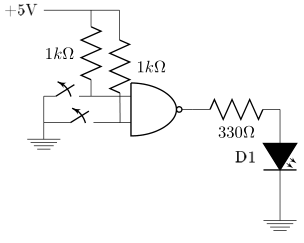
\includegraphics[scale=0.5]{NAND.png}
\caption{Schema circuitale della porta NAND.\label{NAND}}
\label{pin}
\end{figure}

\subparagraph{Circuito AND}
E' stato realizzato il circuito in figura \ref{AND} e la tabella di verità (vedi tabella \refTABELLA), anche in questo caso si è visualizzato l'output sull'oscilloscopio (figura \refFIGURA). Si nota che l'andamento è quello previsto.

\begin{figure}[!htb]
  \centering
  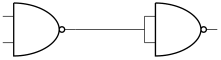
\includegraphics[scale=0.5]{AND.png}
\caption{Schema del circuito AND.\label{AND}}
\label{pin}
\end{figure}

\subparagraph{Circuito OR}
E' stato montato il circuito in figura \ref{OR}. In tabella \refTABELLA è stata rappresentata la tabella di verità e in figura \refFIGURA si può osservare l'andamento dell'output.

\begin{figure}[!htb]
  \centering
  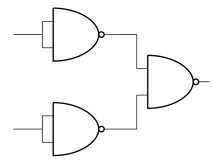
\includegraphics[scale=0.5]{OR.png}
\caption{Schema del circuito OR.\label{OR}}
\label{pin}
\end{figure}

\subparagraph{Circuito XOR}
Abbiamo montato il circuito in figura \ref{XOR}, scritto la tabella di verità (tabella \ref)e osservato l'output sull'oscilloscopio (figura \ref).

\begin{figure}[!htb]
  \centering
  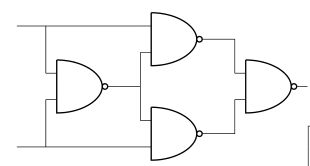
\includegraphics[scale=0.5]{XOR.png}
\caption{Schema del circuito XOR.\label{XOR}}
\label{pin}
\end{figure}

\subparagraph{Circuito sommatore a un bit}
Il circuito sommatore a un bit in figura \ref{sommatore} è stato montato aggiungendo al circuito XOR un NOT. Anche in questo caso abbiamo scritto la tabella di verità (tabella \ref) e visualizzato l'output con l'oscilloscopio (figura \ref).

\begin{figure}[!htb]
  \centering
  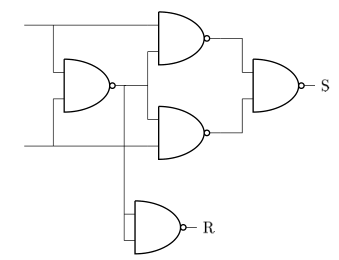
\includegraphics[scale=0.5]{sommatore.png}
\caption{Schema del circuito sommatore a un bit.\label{sommatore}}
\label{pin}
\end{figure}


\section{Multivibratore monostabile}
Abbiamo montato il circuito in figura \ref{monostabile}. I componenti sono stati misurati con il multimetro digitale e risultano essere $R_1= $ e $C= $. Si è scelta come corrente di alimentazione $V_{CC}= $ e come frequenza dell'onda quadra inviata dal circuito pulsatore $f= $, ottenendo così un \emph{duty cycle} pari a TOT e una tensione massima di TOT. 

%osservare V_IN, V_C e V_OUT con l'oscilloscopio
% vedere che variando l'impulso input, impulso output non cambia se in è minore di out
%spiegazione teorica e immagini
%cambiare R_1 e fit lineare R_1 vs durata impulso in uscita

\begin{figure}[!htb]
  \centering
  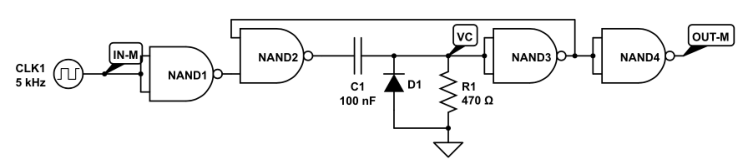
\includegraphics[scale=0.5]{monostabile.png}
\caption{Schema del circuito multivibratore monostabile.\label{monostabile}}
\label{pin}
\end{figure}


\section{Multivibratore astabile}
Abbiamo montato il circuito in figura \ref{astabile}, misurando con il multimetro digitale $R_2= $, $C_2= $ e $V_{CC}= $. Si sono osservati all'oscilloscopio $V_{C,2}= $ e $V_{OUT}= $, quindi abbiamo misurato il periodo in uscita $T= $ e \emph{duty cycle} pari a TOT.
%spiegazione circuito e immagini oscilloscopio
Come per il circuito multivibratore monostabile abbiamo variato il valore della resistenza per verificare la dipendenza lineare tra $R_2$ e il tempo di durata dell'impulso in uscita t, quindi abbiamo eseguito un \emph{fit} lineare e ottenuto TOT.
%tabella e fit

\begin{figure}[!htb]
  \centering
  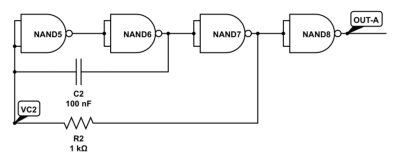
\includegraphics[scale=0.5]{astabile.png}
\caption{Schema del circuito multivibratore astabile.\label{astabile}}
\label{pin}
\end{figure}

\section{Generatore di onda quadra}
Il multivibratore astabile è stato collegato al monostabile tramite un derivatore, in modo da ottenere il generatore di onda quadra in figura \ref{generatorequadra}. 

%spiegazione teorica
%immagini
%variare le resistenze e vedere la dipendenza lineare con il periodo dell'impulso in uscita.

\begin{figure}[!htb]
  \centering
  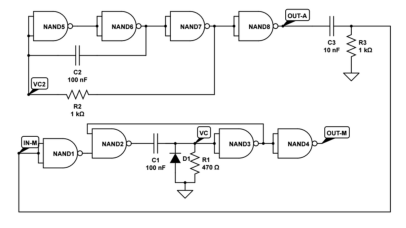
\includegraphics[scale=0.5]{generatorequadra.png}
\caption{Schema del generatore di onda quadra.\label{generatorequadra}}
\label{pin}
\end{figure}

\end{document}